\subsubsection{\texttt{RF-1}: registro de profesores por invitación}
\label{subsec:rf1}

En la versión de \textit{VSCode4Teaching} tomada como punto de partida, mientras que los estudiantes gozaban de libertad total para poder crear una cuenta en la aplicación a través de la extensión, los profesores debían ser registrados manualmente por otros profesores, evitando así que estudiantes o personal no acreditado pudiese tener cuenta con privilegios de docente. Esto conllevaba que los profesores con cuenta preexistente tuviesen que introducir manualmente el nombre, apellidos, correo electrónico, nombre de usuario y contraseña de los nuevos docentes, generando un riesgo de seguridad ---ya que no es posible modificar la contraseña una vez establecida---.

Como consecuencia, se ha modificado este proceso para ``invertir'' su funcionamiento, de modo que los profesores pueden generar invitaciones para otros docentes introduciendo su nombre, apellidos, correo electrónico y nombre de usuario. Una vez generada la invitación, que tiene forma de enlace a una página web ---con el aspecto visual reflejado en la \referenciaFigura{fig:reqf1-1}---, puede remitírsela al docente invitado, quien puede acceder al enlace en un navegador web para, introduciendo su nombre de usuario como método de verificación, escoger la contraseña de su elección sin necesidad de comunicársela a ninguna otra persona.

Esta es una de las funcionalidades que aprovecha la introducción de la nueva aplicación web SPA introducida como cliente adicional del servidor ---tal como figura en la \referenciaSeccion{sec:diseñoArquitectura}---, ya que el docente invitado accede mediante el enlace suministrado a un asistente implementado dentro de esta aplicación web ---y no en la extensión---.

\begin{figure}[ht]
    \centering
    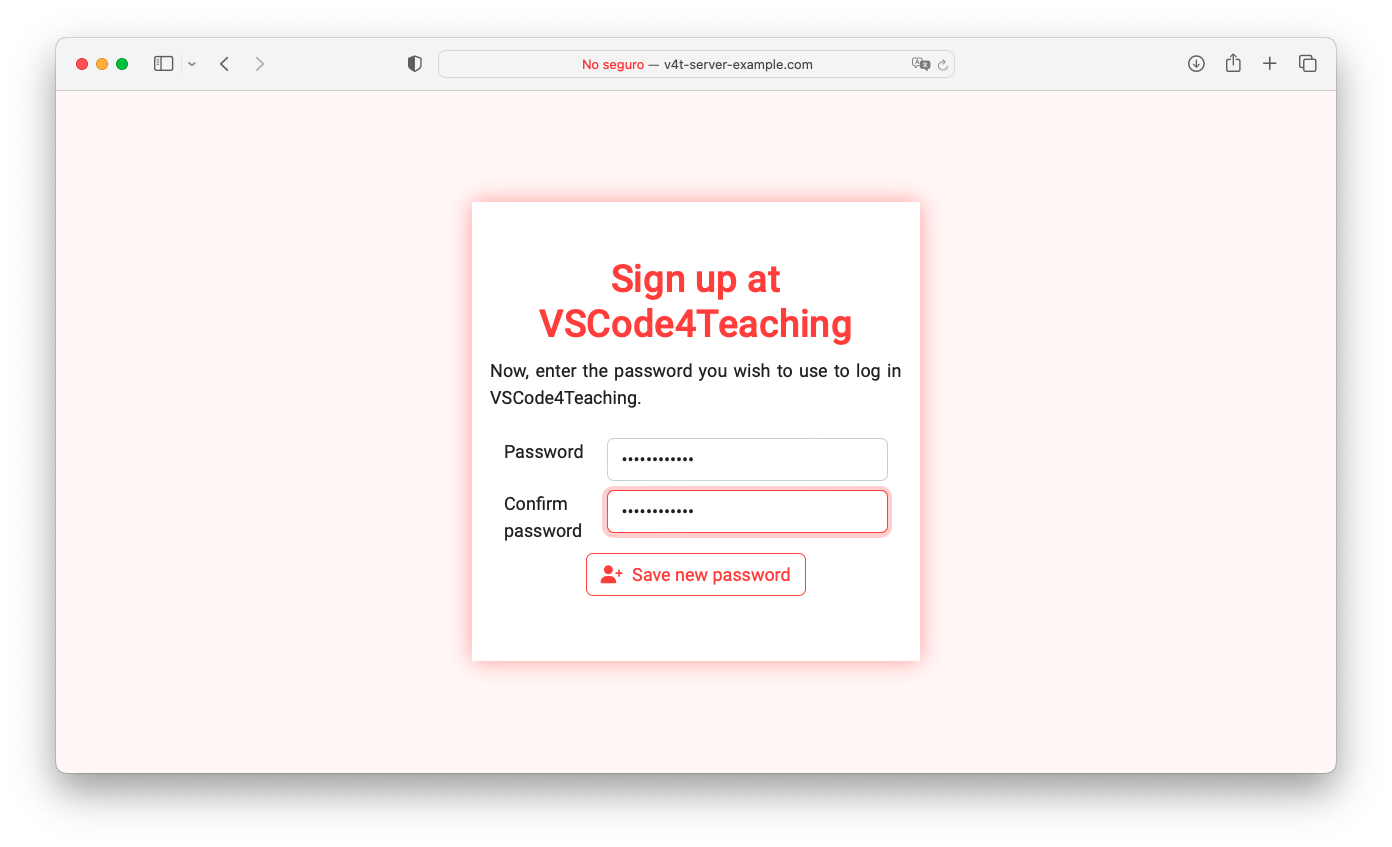
\includegraphics[width=\textwidth]{imagenes/utilizadas/4-3-implementacion/rf1-1.png}
    \caption{Captura del navegador web durante el proceso de configuración de contraseña de un nuevo profesor.}
    \label{fig:reqf1-1}
\end{figure}
